%!TEX root = ../article.tex

\section{Background}
\label{sec:background}
In this section we will provide an overview of the relevant related work to solve the challenges of
converging the Internet of Things and Utility Computing. The most relevant concepts necessary to
understand our proposal will be described throughout this section.

% Cloud computing concepts and tools
\subsection{Cloud computing concepts and tools}
\label{sub:cloud_concepts_tools}

% Smart Place Deployment
\subsubsection{Smart Place Deployment}
\label{sub:smart_place_deployment}
Deployment of smart places usually was performed in a physical and isolated manner. By leveraging the
infrastructure of smart places to the cloud, new provisioning approaches have to be adopted. Currently,
cloud service delivery models are being developed based on the existing layers of the cloud
architecture \cite{zhang2010cloud}: \textit{IaaS}, \textit{PaaS} and \textit{SaaS}.\\

% Distefano
Distefano et al. \cite{distefano2012enabling} proposed a conceptual architecture by
mapping various elements in both cloud and IoT to the three layers of the cloud architecture (\gls{IaaS},
\gls{PaaS} and \gls{SaaS}). In this proposal IoT resources are provided voluntarily by their owners,
while management functions - such as node management and policy enforcement - are viewed as peer
functions of cloud infrastructure management. A \gls{PaaS} module is responsible to mashup IoT and
cloud infrastructure (\gls{IaaS}) resources for applications, which are delivered to the clients
through \gls{SaaS}.
% CloudThings
CloudThings \cite{zhou2013cloudthings} is an architecture that uses the cloud platform layers to
integrate Internet of Things and Cloud Computing. The proposed architecture is an online platform
which accommodates \gls{IaaS}, \gls{PaaS}, \gls{SaaS} and allows system integrators and solution
providers to leverage the complete application infrastructure for developing, operating and composing
applications and services.
% IoT PaaS
Li et. al \cite{li2013efficient} proposed IoT PaaS, a cloud platform that supports
scalable IoT service delivery. Solution providers are able to deliver new solutions by leveraging
computing resources and platform services - domain mediation, application context management, etc.
- to the cloud. The proposed architecture aims to enable virtual vertical service delivery, for that
it has a multi-tenant nature which is designed to help at the isolation of the environments of
different solutions.\\

Although a significant progress was achieved regarding the improvement for the deployment of \gls{IoT}
solutions, most of the work still are in a conceptual stage. What is certain is that cloud service
delivery models will be the basis for the service delivery models of \gls{IoT} solutions.\\

% Configuration Management Tools
\subsubsection{Configuration Management Tools}
\label{subs:cm_tools}
\gls{CM} tools are software management tools that allows to automate and specify the deployment of an
application. Usually, users describe the system resources and their desired state and the \gls{CM}
tool is responsible for enforcing the desired state. For instance, \gls{CM} tools allows the automation
of the provisioning of physical and virtual machines, perform dependency management of software
components and to perform the automation of management tasks. Currently, there are several solutions
to perform configuration management of software, where the most relevant are Chef\footnote{\url{https://www.chef.io/}},
Puppet\footnote{\url{https://puppetlabs.com/}}, Ansible\footnote{\url{http://www.ansible.com/}} and
Salt\footnote{\url{http://saltstack.com/}}.\\

% Fog Computing
\subsection{Fog computing for low latency responses}
\label{sub:fog_computing}
The Fog Computing \cite{bonomi2012fog} is a platform that aims to bring the cloud close to the ``edge
of the Network''. By bringing the cloud close to the ground - hence the fog analogy - the Fog will be
able to meet the requirements of several applications that the traditional clouds are not able to
accomplish. The most notable case is the Internet of Things, that requires mobility support,
geo-distribution in addition to location awareness and low latency. The Fog aims to achieve that by
virtualizing the computing, storage and network services between end devices and the
traditional data centers in the cloud.\\

% Fog Computing Infrastructure
\begin{figure}[ht!]
  \centering
  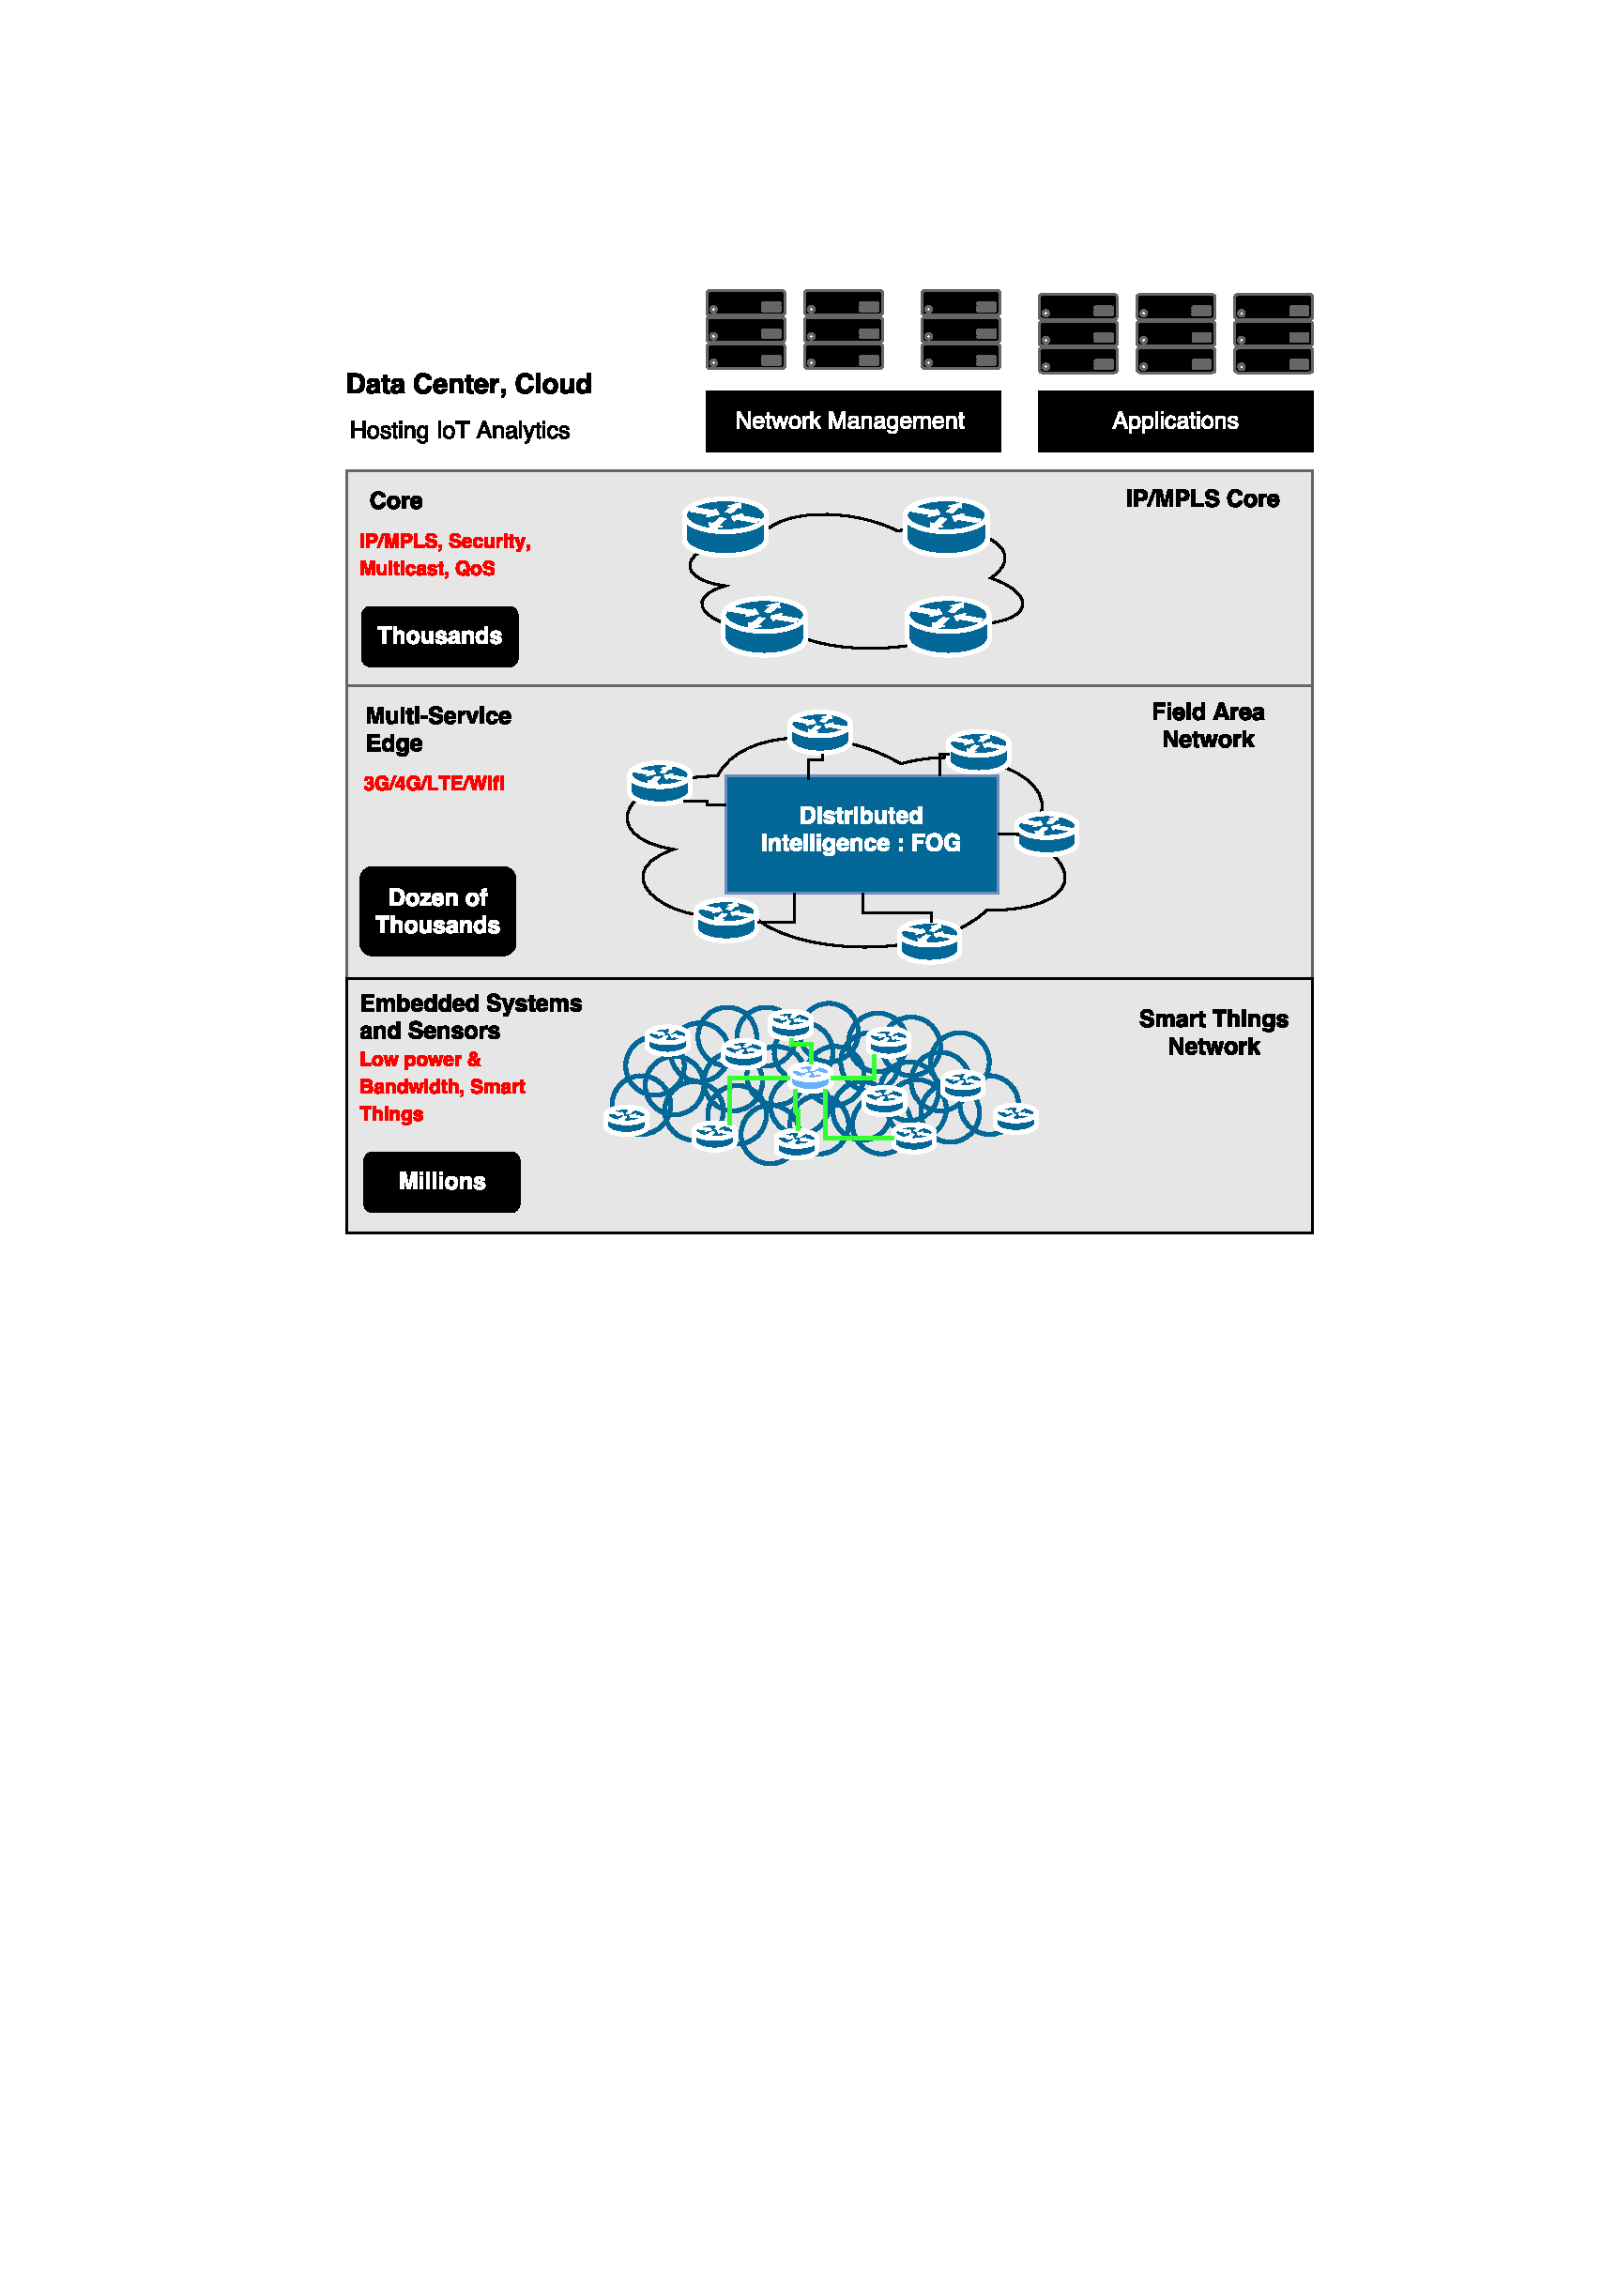
\includegraphics[width=.5\textwidth]{./figures/fog_architecture}
  \caption[IoT and Fog Computing.]{The Internet of Things and Fog Computing (Bonomi et. al (2012)).}
  \label{fig:fog_architecture}
\end{figure}

Bonomi et. al \cite{bonomi2012fog} presents the architecture of a Fog Computing platform. As illustrated
in Figure~\cite{bonomi2012fog} the distributed infrastructure of the Fog comprising of several players,
covering from data centers, core of the network, edge of the network and end devices. The \textit{Embedded Systems and Sensors}
is the lowest tier of the Fog and it is responsible for performing \gls{M2M} interactions. It collects and
process the data from the sensors, issues commands to the actuators and also filters the data that
is locally consumed and sent to the higher tiers. The \textit{Multi-Service Edge} and \textit{Core}
tiers are responsible for performing visualization and reporting - e.g. \gls{H2M} interaction -
as well to deal with systems and processes (\gls{M2M}).\\

Since the interaction time between the different tiers can range from seconds - e.g. low-latency real-time
analytics - to days - transactional analytics - the Fog must support several types of storage, from
ephemeral storage at the lowest tiers to semi-permanent at the highest tier. As higher is the tier,
geographical coverage and the time scale increases \cite{bonomi2014fog}. The global coverage
is given by the Cloud, which acts as a central repository for the persistent data and that is used
to perform business analytics.

% Fosstrak
\subsection{Fosstrak Platform}
\label{sub:fosstrak}
The Free and Open Source Software for Track and Trace (Fosstrak) is an EPCglobal Network compliant
\gls{RFID} software platform that was developed by Floerkemeier et. al \cite{floerkemeier2007rfid}.
Figure~\ref{fig:fosstrak_architecture} presents the architecture of the Fosstrak platform.\\

% Fosstrak Architecture
\begin{figure}[ht!]
  \centering
  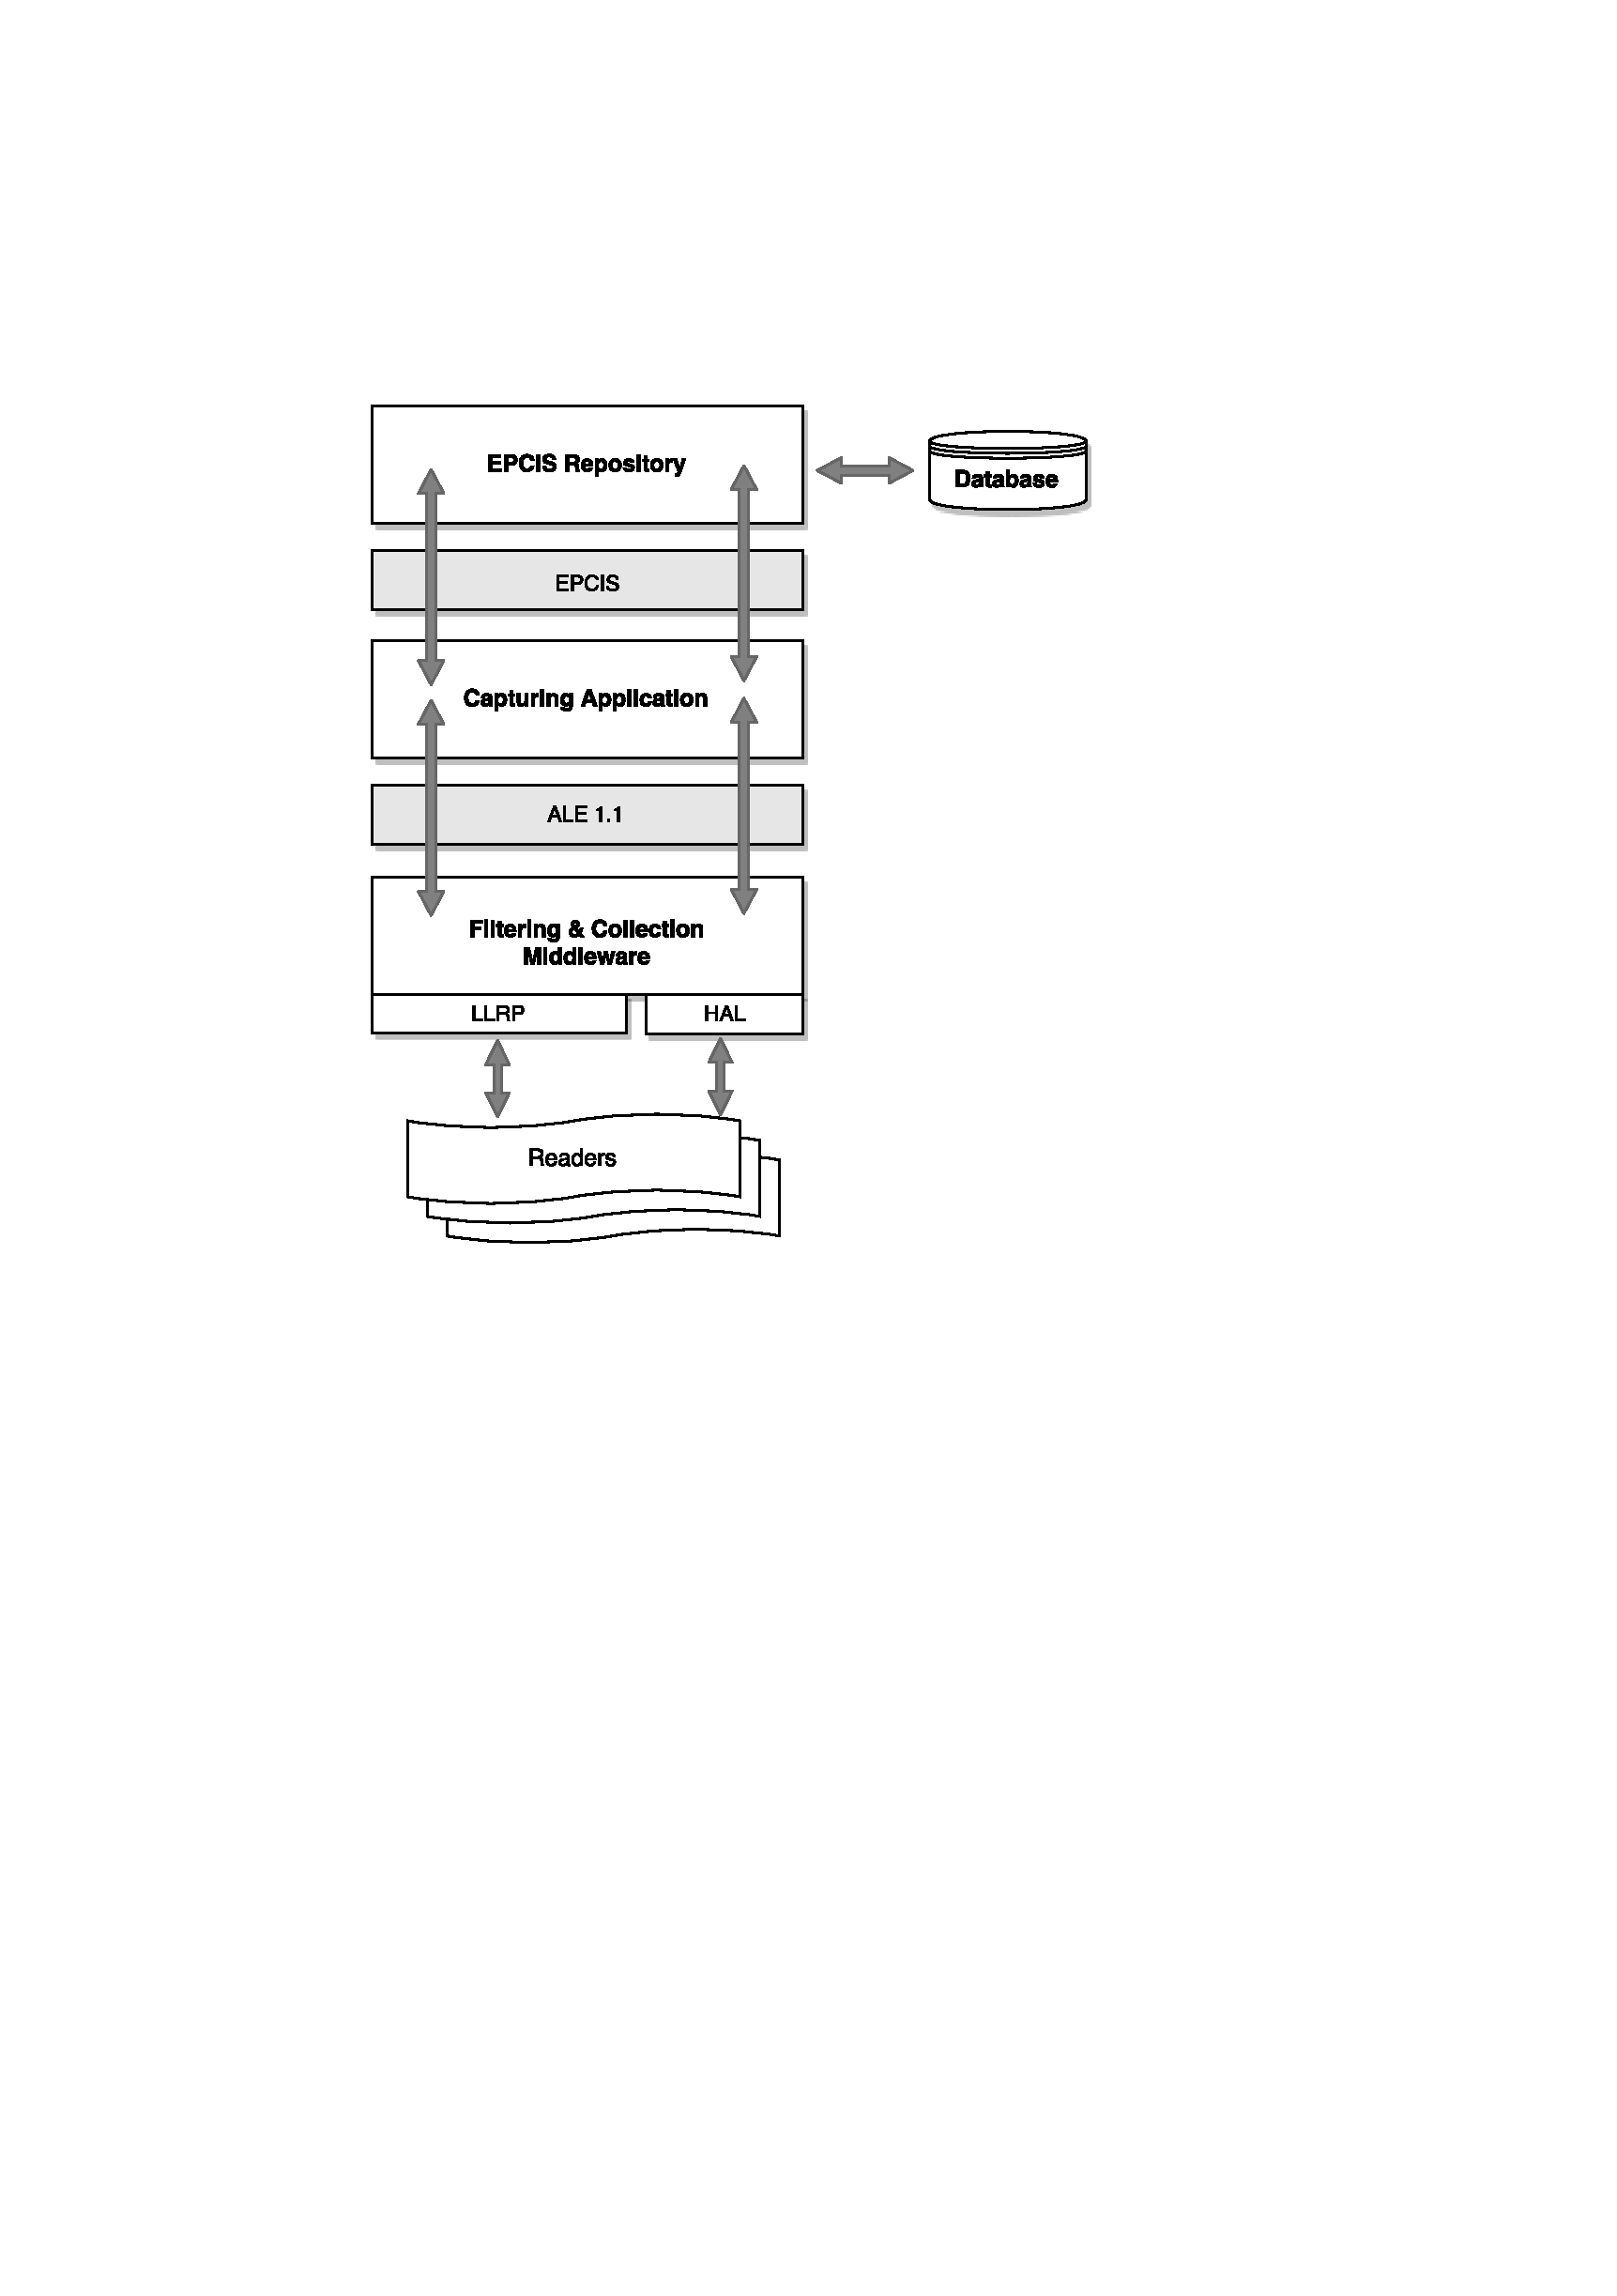
\includegraphics[width=.45\textwidth]{./figures/fosstrak_architecture}
  \caption[Fosstrak architecture.]{Fosstrak architecture.}
  \label{fig:fosstrak_architecture}
\end{figure}

The Fosstrak platform is composed by the following modules: \textit{a) Filtering \& Collection Server}
is the module responsible for filtering and collecting data from \gls{RFID} readers. The module uses the
\gls{LLRP} and \gls{HAL} interfaces to communicate with readers; \textit{b) Capturing Application} is
the module responsible for transforming uninterpreted events into meaningful business events; and
\textit{c) EPCIS Repository} is the module that provides persistence for \gls{EPCIS} events.
